\chapter{Continuous time Markov processes}

\section{Lotka--Volterra model}

\begin{sourcefiles}
  \item[Source codes] src/071\_lotka\_volterra.c, src/ctmp/gillespie.h,
    src/ctmp/gillespie.c, src/ctmp/lotka\_volterra.h
  \item[Analysis script] src/071\_lotka\_volterra.R
  \item[Executables] exe/071\_lotka\_volterra 
\end{sourcefiles}

For this exercise and the next, I wrote a generic implementation of the
Gillespie algorithm, found in \texttt{src/ctmp/gillespie.c}. The header file
\texttt{src/ctmp/lotka\_volterra.h} implements the specific rate and update
functions for the Lotka--Volterra model. Then I ran a set of simulations fixing
the three parameters to $k_{1} = \qty{3}{\per\second}$ (prey birth rate), $k_{2}
= \qty{0.01}{\per\second}$ (predation rate) and $k_{3} = \qty{5}{\per\second}$
(predators death rate); the results are in \cref{fig:071a,fig:071b}.

\begin{figure}
  \centering
  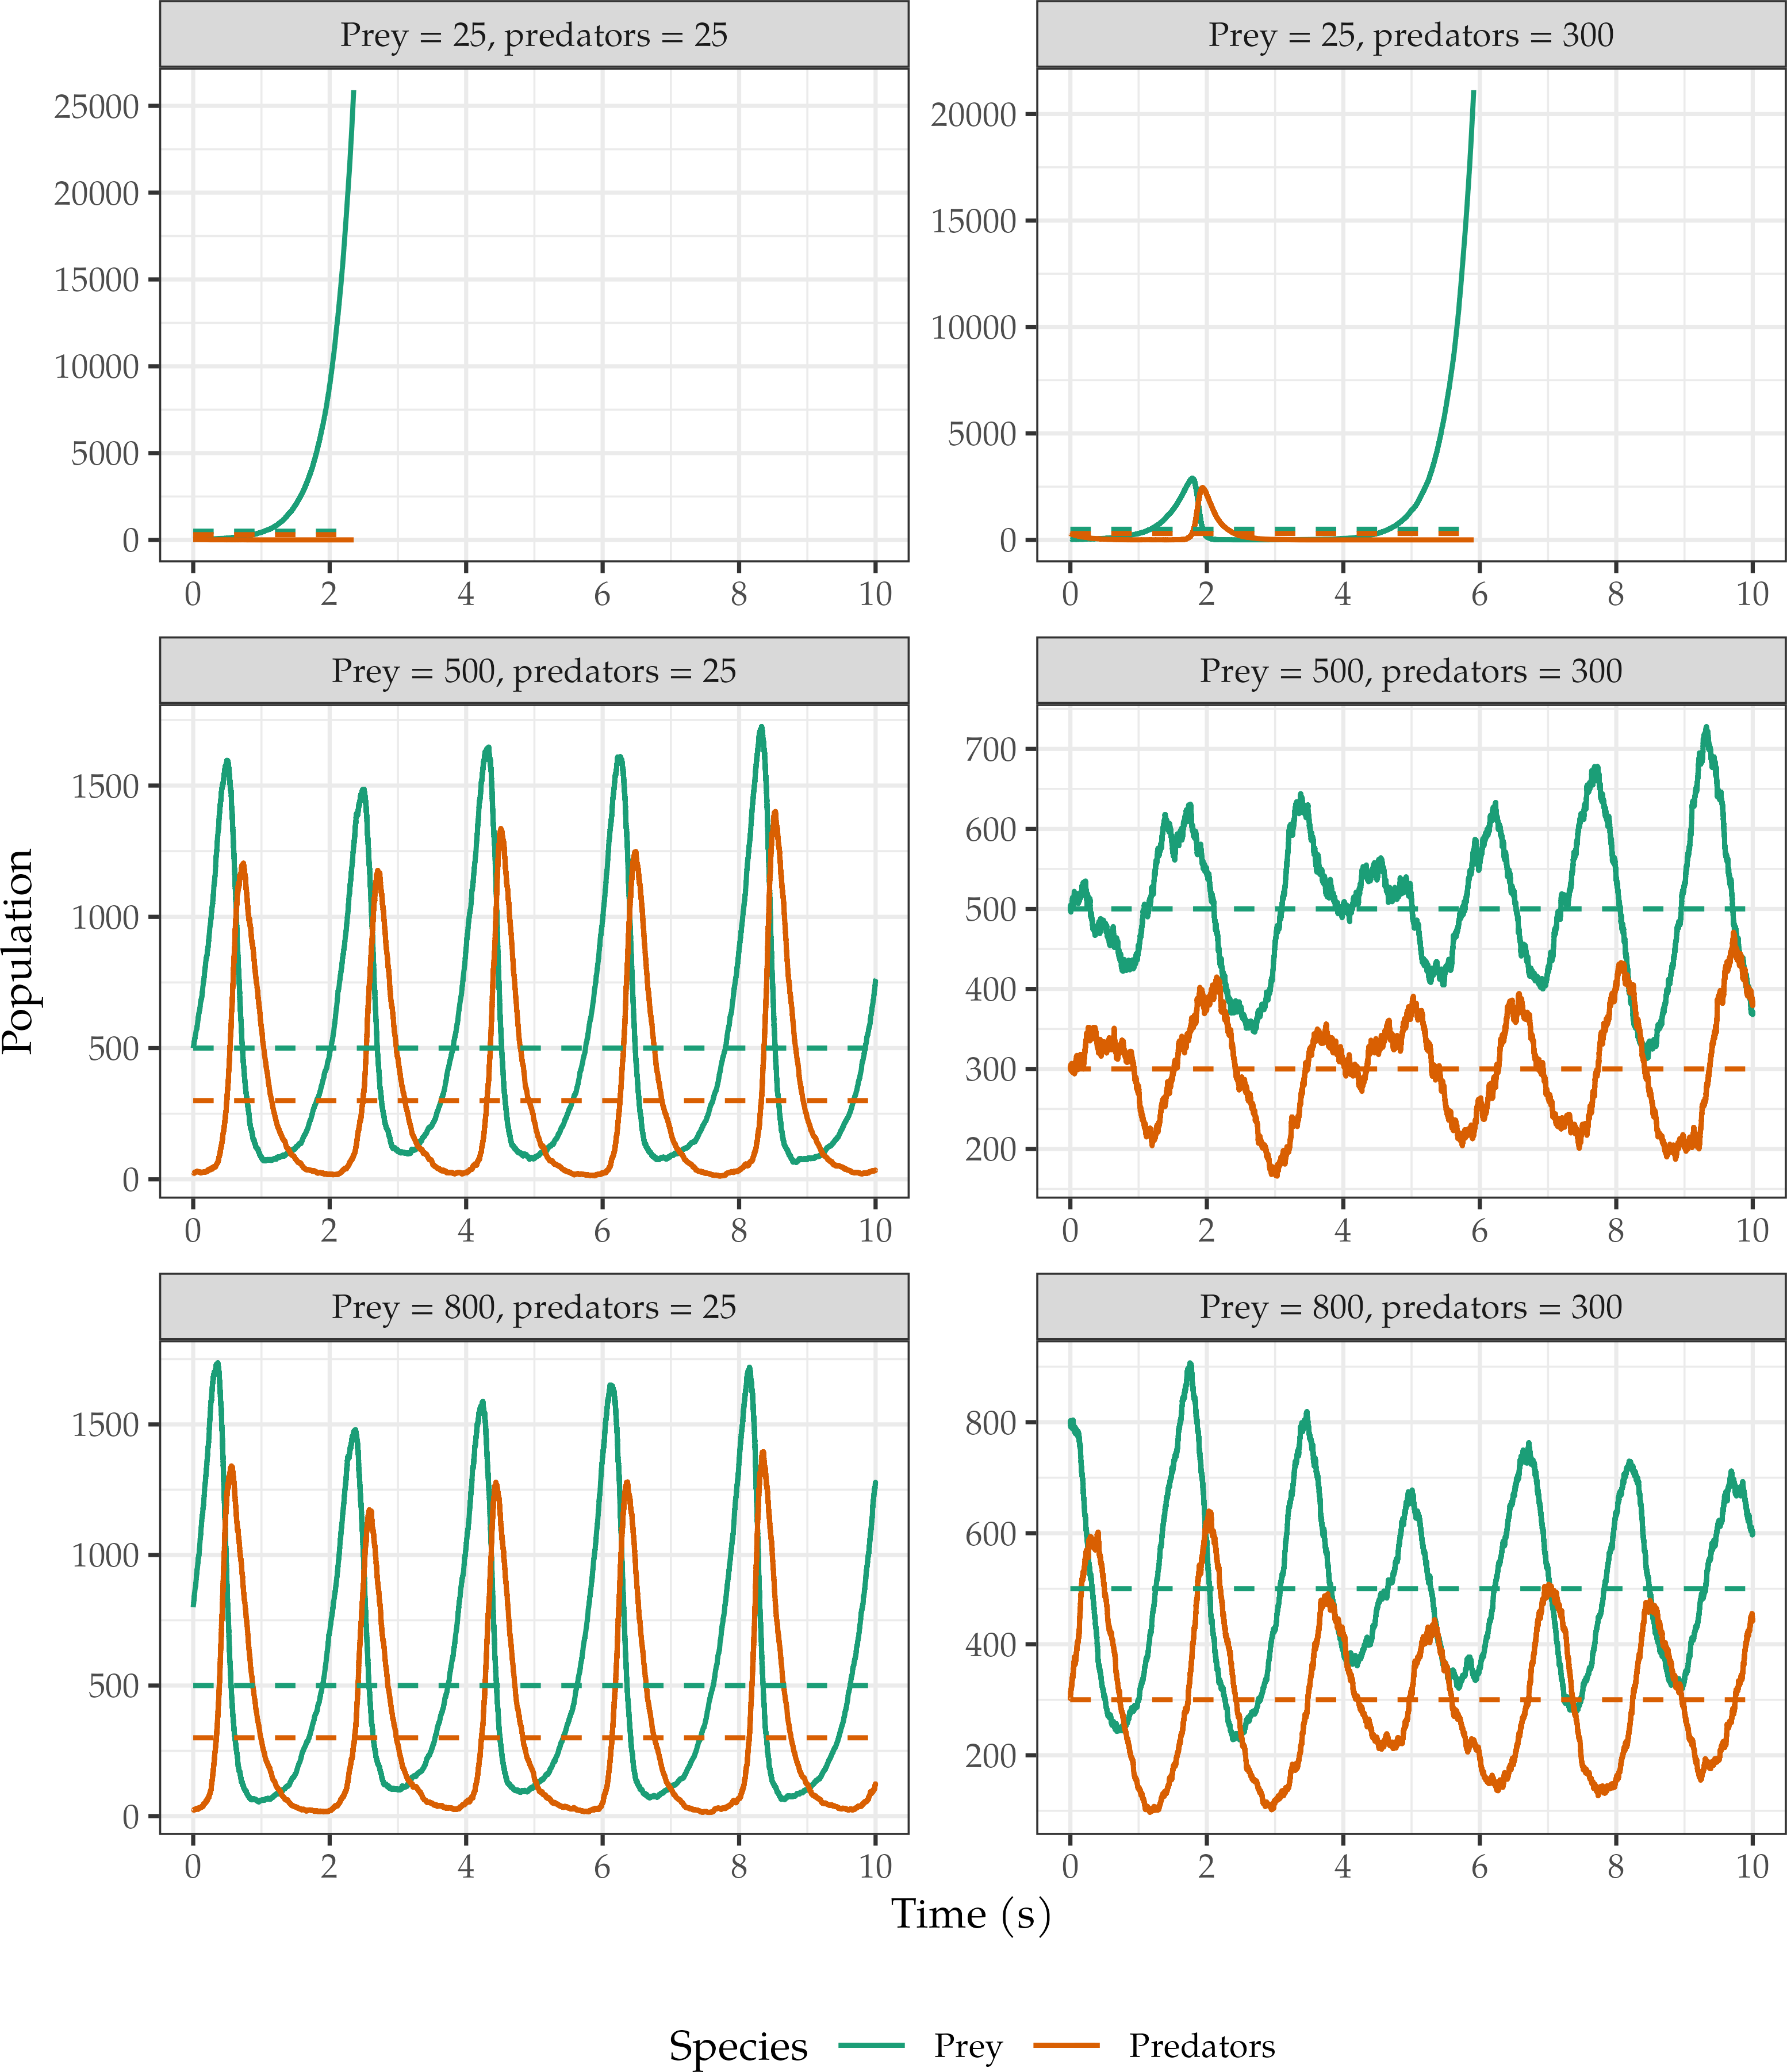
\includegraphics{img/071a.png}
  \caption{first set of Lotka--Volterra simulations with $k_{1} =
    \qty{3}{\per\second}$, $k_{2} = \qty{0.01}{\per\second}$ and $k_{3} =
    \qty{5}{\per\second}$. The initial conditions are reported above each plot
    and the stationary solution $(k_{3} / k_{2}, k_{1} / k_{2})$ is highlighted
    with dashed lines.}
  \label{fig:071a}
\end{figure}

\begin{figure}
  \centering
  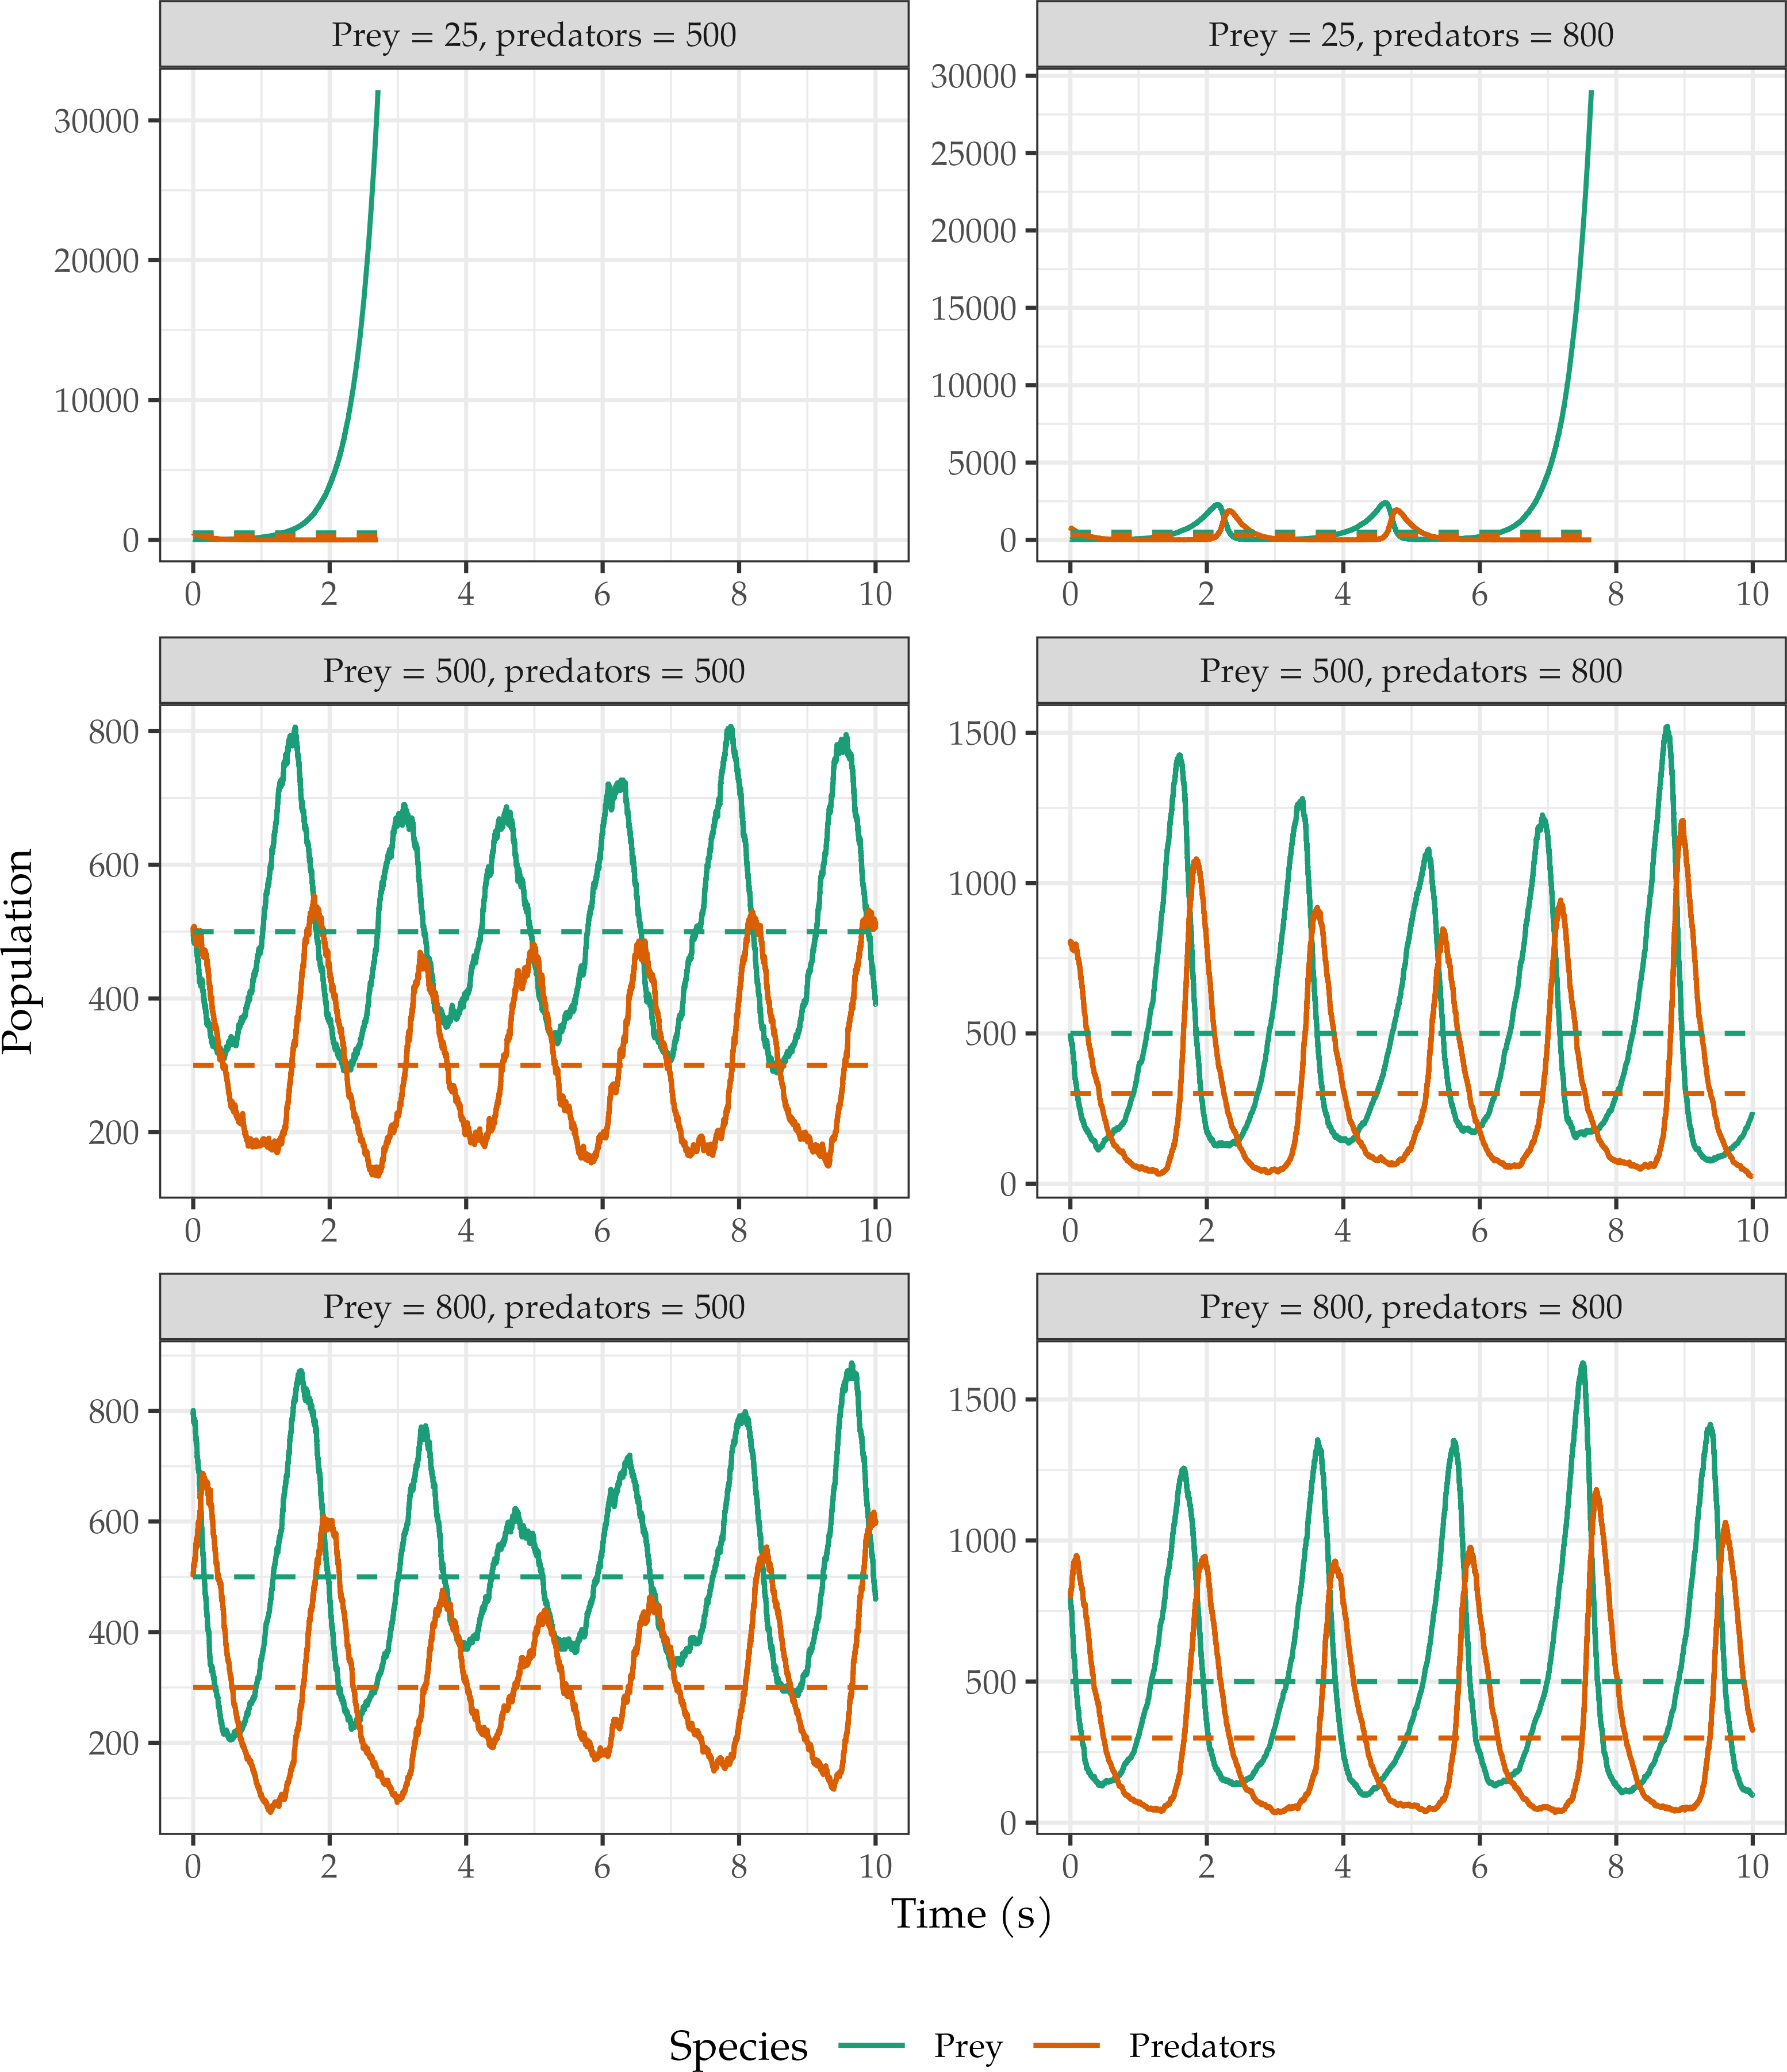
\includegraphics{img/071b.png}
  \caption{second set of Lotka--Volterra simulations with $k_{1} =
    \qty{3}{\per\second}$, $k_{2} = \qty{0.01}{\per\second}$ and $k_{3} =
    \qty{5}{\per\second}$. The initial conditions are reported above each plot
    and the stationary solution $(k_{3} / k_{2}, k_{1} / k_{2})$ is highlighted
    with dashed lines.}
  \label{fig:071b}
\end{figure}

The non-trivial stationary solution is $(k_{3} / k_{2}, k_{1} / k_{2})$, which
equals $(\num{500}, \num{300})$ with this choice of parameters. When the initial
condition is close to this equilibrium point, as shown in the right middle panel
of \cref{fig:071a} or the left middle panel of \cref{fig:071b}, the oscillations
can be relatively small and almost sinusoidal, with the predators' trend
mirroring that of the prey but with a delay. However, when one or both initial
populations are very far from the $(\num{500}, \num{300})$ point, as in the left
bottom panel of \cref{fig:071a} or the bottom right panel of \cref{fig:071b},
the oscillations become more pronounced and take on a characteristic shape. In
this case, in addition to the delay in the predators' trend, a sharp peak in
both populations is followed by a drop -- first of the prey population, which
quickly recovers, and then of the predators, which recover only when the prey
population reaches a new maximum.

When food is scarce, predators may go extinct and prey grow exponentially with
rate $k_{1}$ -- this happens in the two upper panels of both \cref{fig:071a} and
\cref{fig:071b}. Predator extinction can also be prevented by decreasing the
predator death rate and/or increasing the predation rate, provided that both the
prey birth rate and predator death rate remain sufficiently high -- otherwise,
over-predation would drive the prey to extinction. For example, \cref{fig:071c}
shows a combination of parameters, $k_{1}$ and $k_{2}$ as before but $k_{3}$
lowered to \qty{4}{\per\second}, that easily leads to a \enquote{well-behaved}
solution. But if we further lower the predator death rate to
\qty{2}{\per\second}, the predators can easily grow too quickly, leading to the
extinction of both species, as shown in \cref{fig:071d}.

\begin{figure}
  \centering
  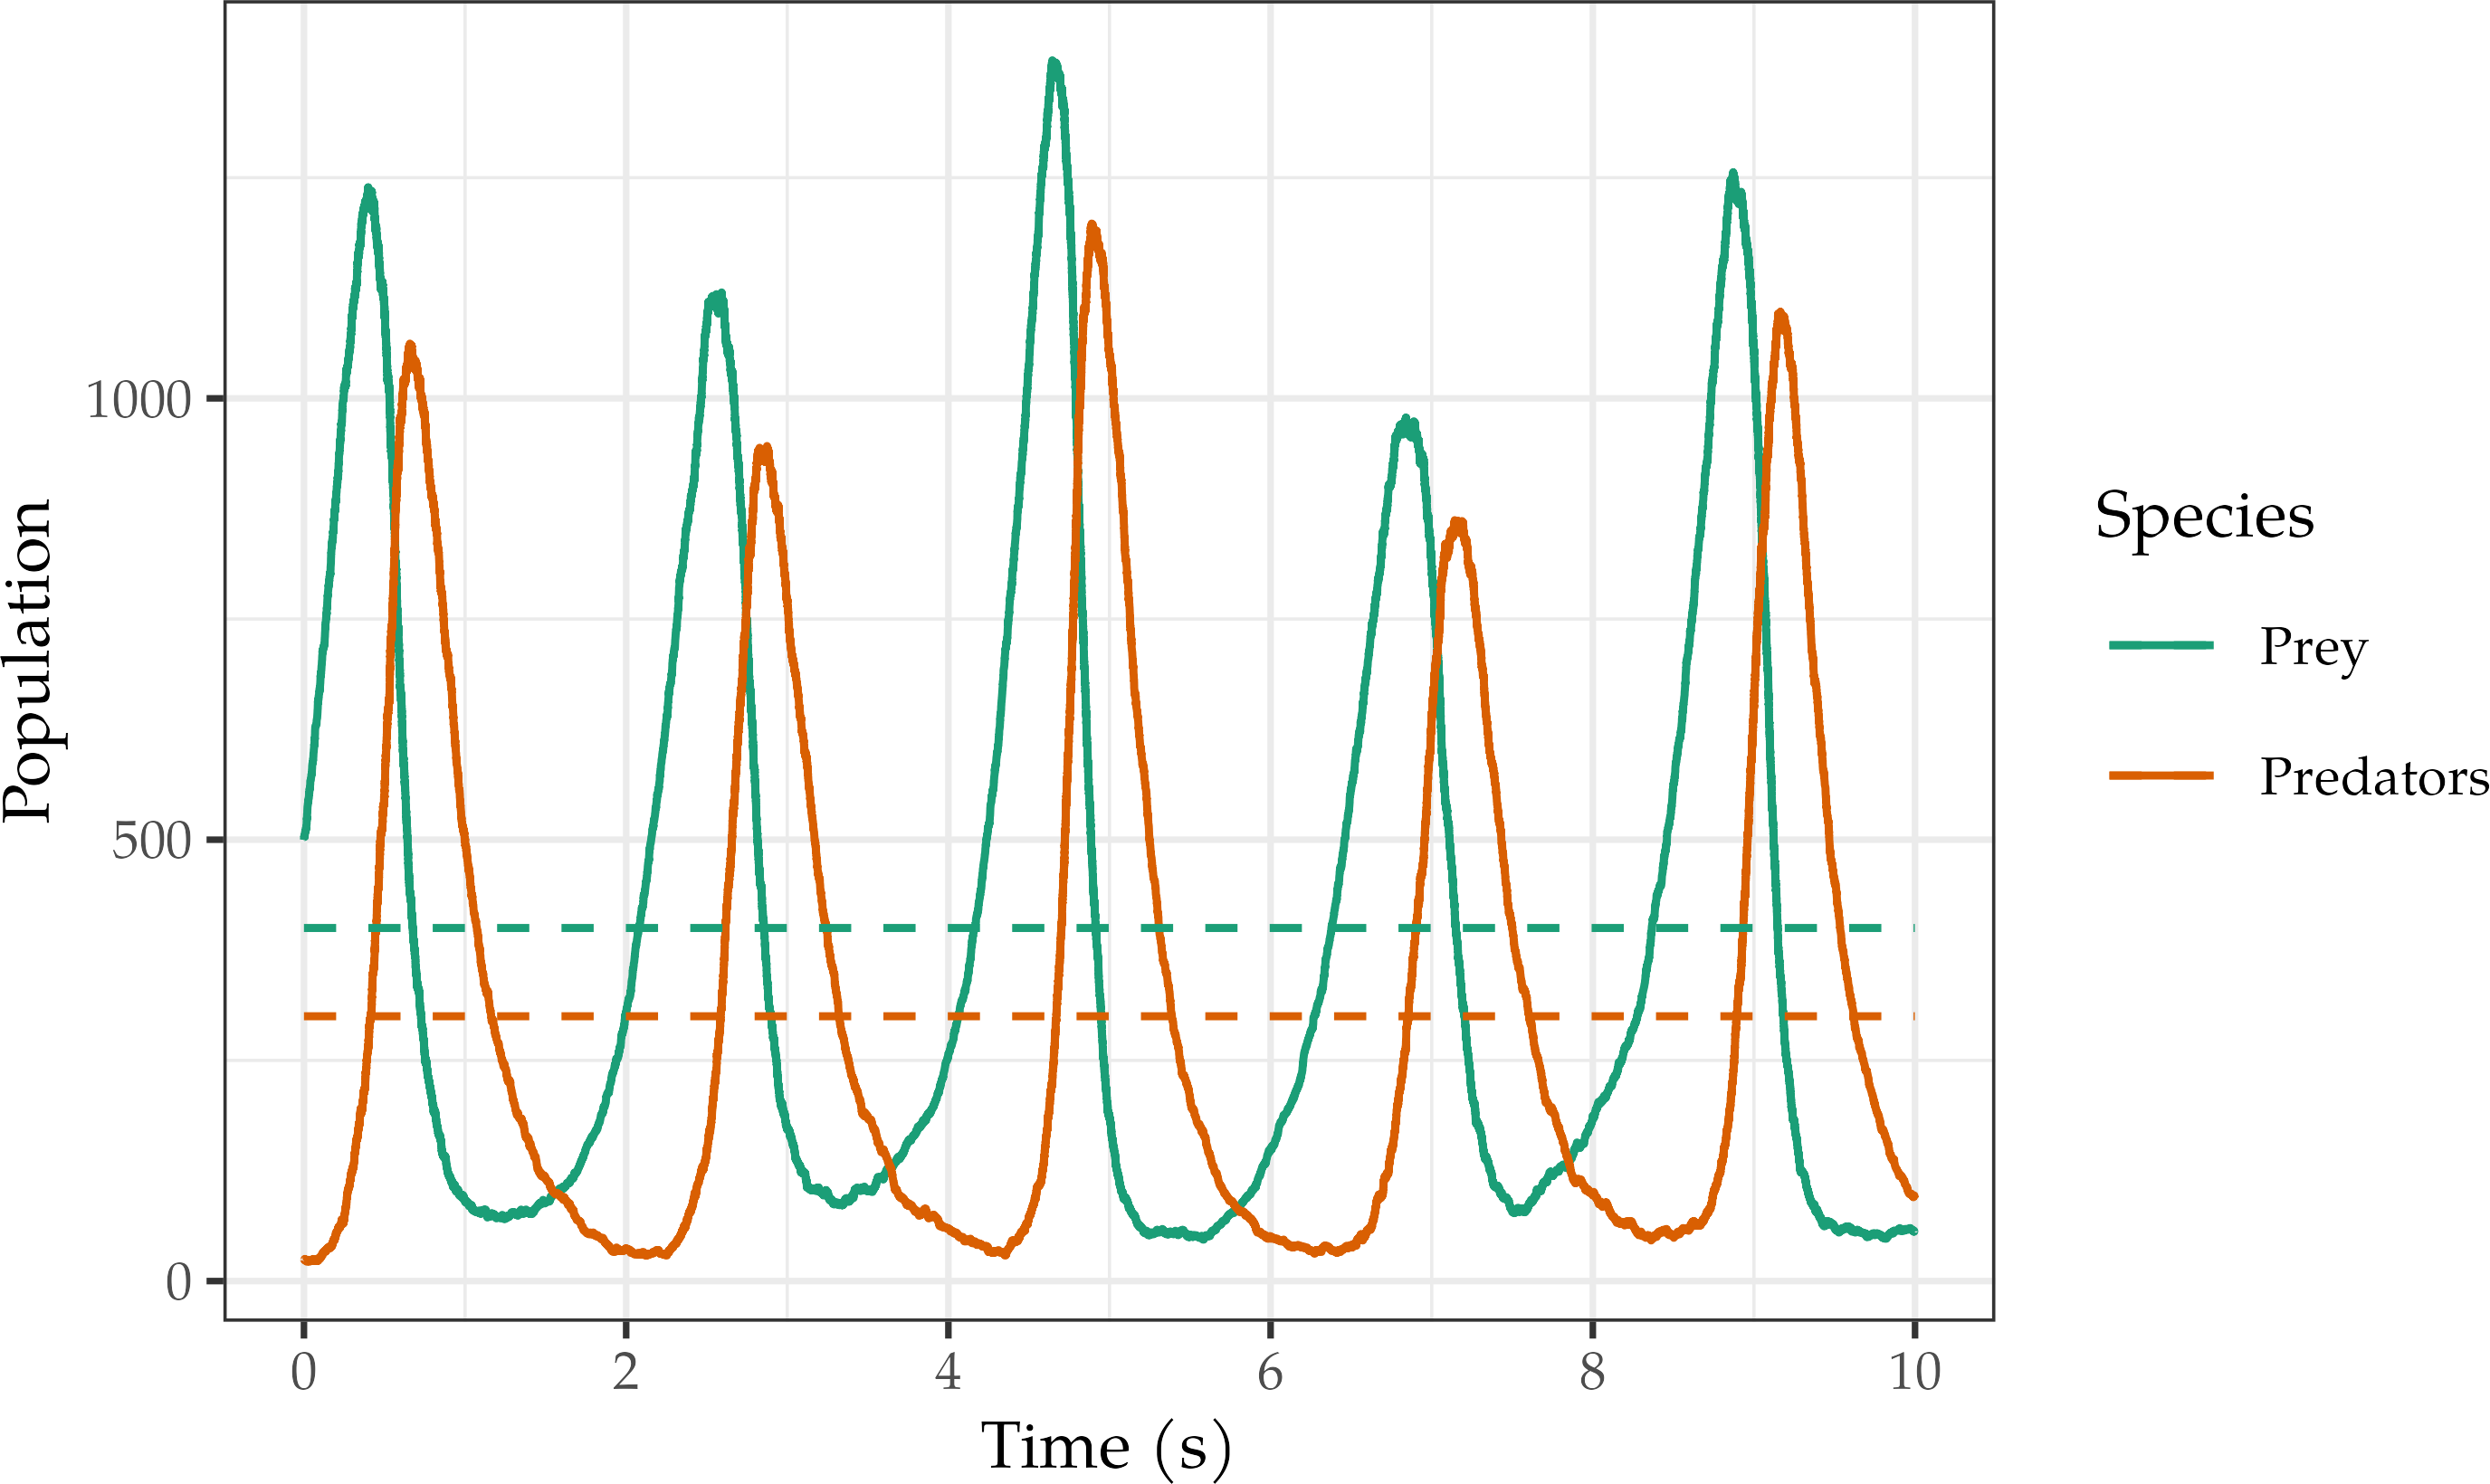
\includegraphics{img/071c.png}
  \caption{simulation of the Lotka--Volterra model with $k_{1} =
    \qty{3}{\per\second}$, $k_{2} = \qty{0.01}{\per\second}$ and $k_{3} =
    \qty{4}{\per\second}$.}
  \label{fig:071c}
\end{figure}

\begin{figure}
  \centering
  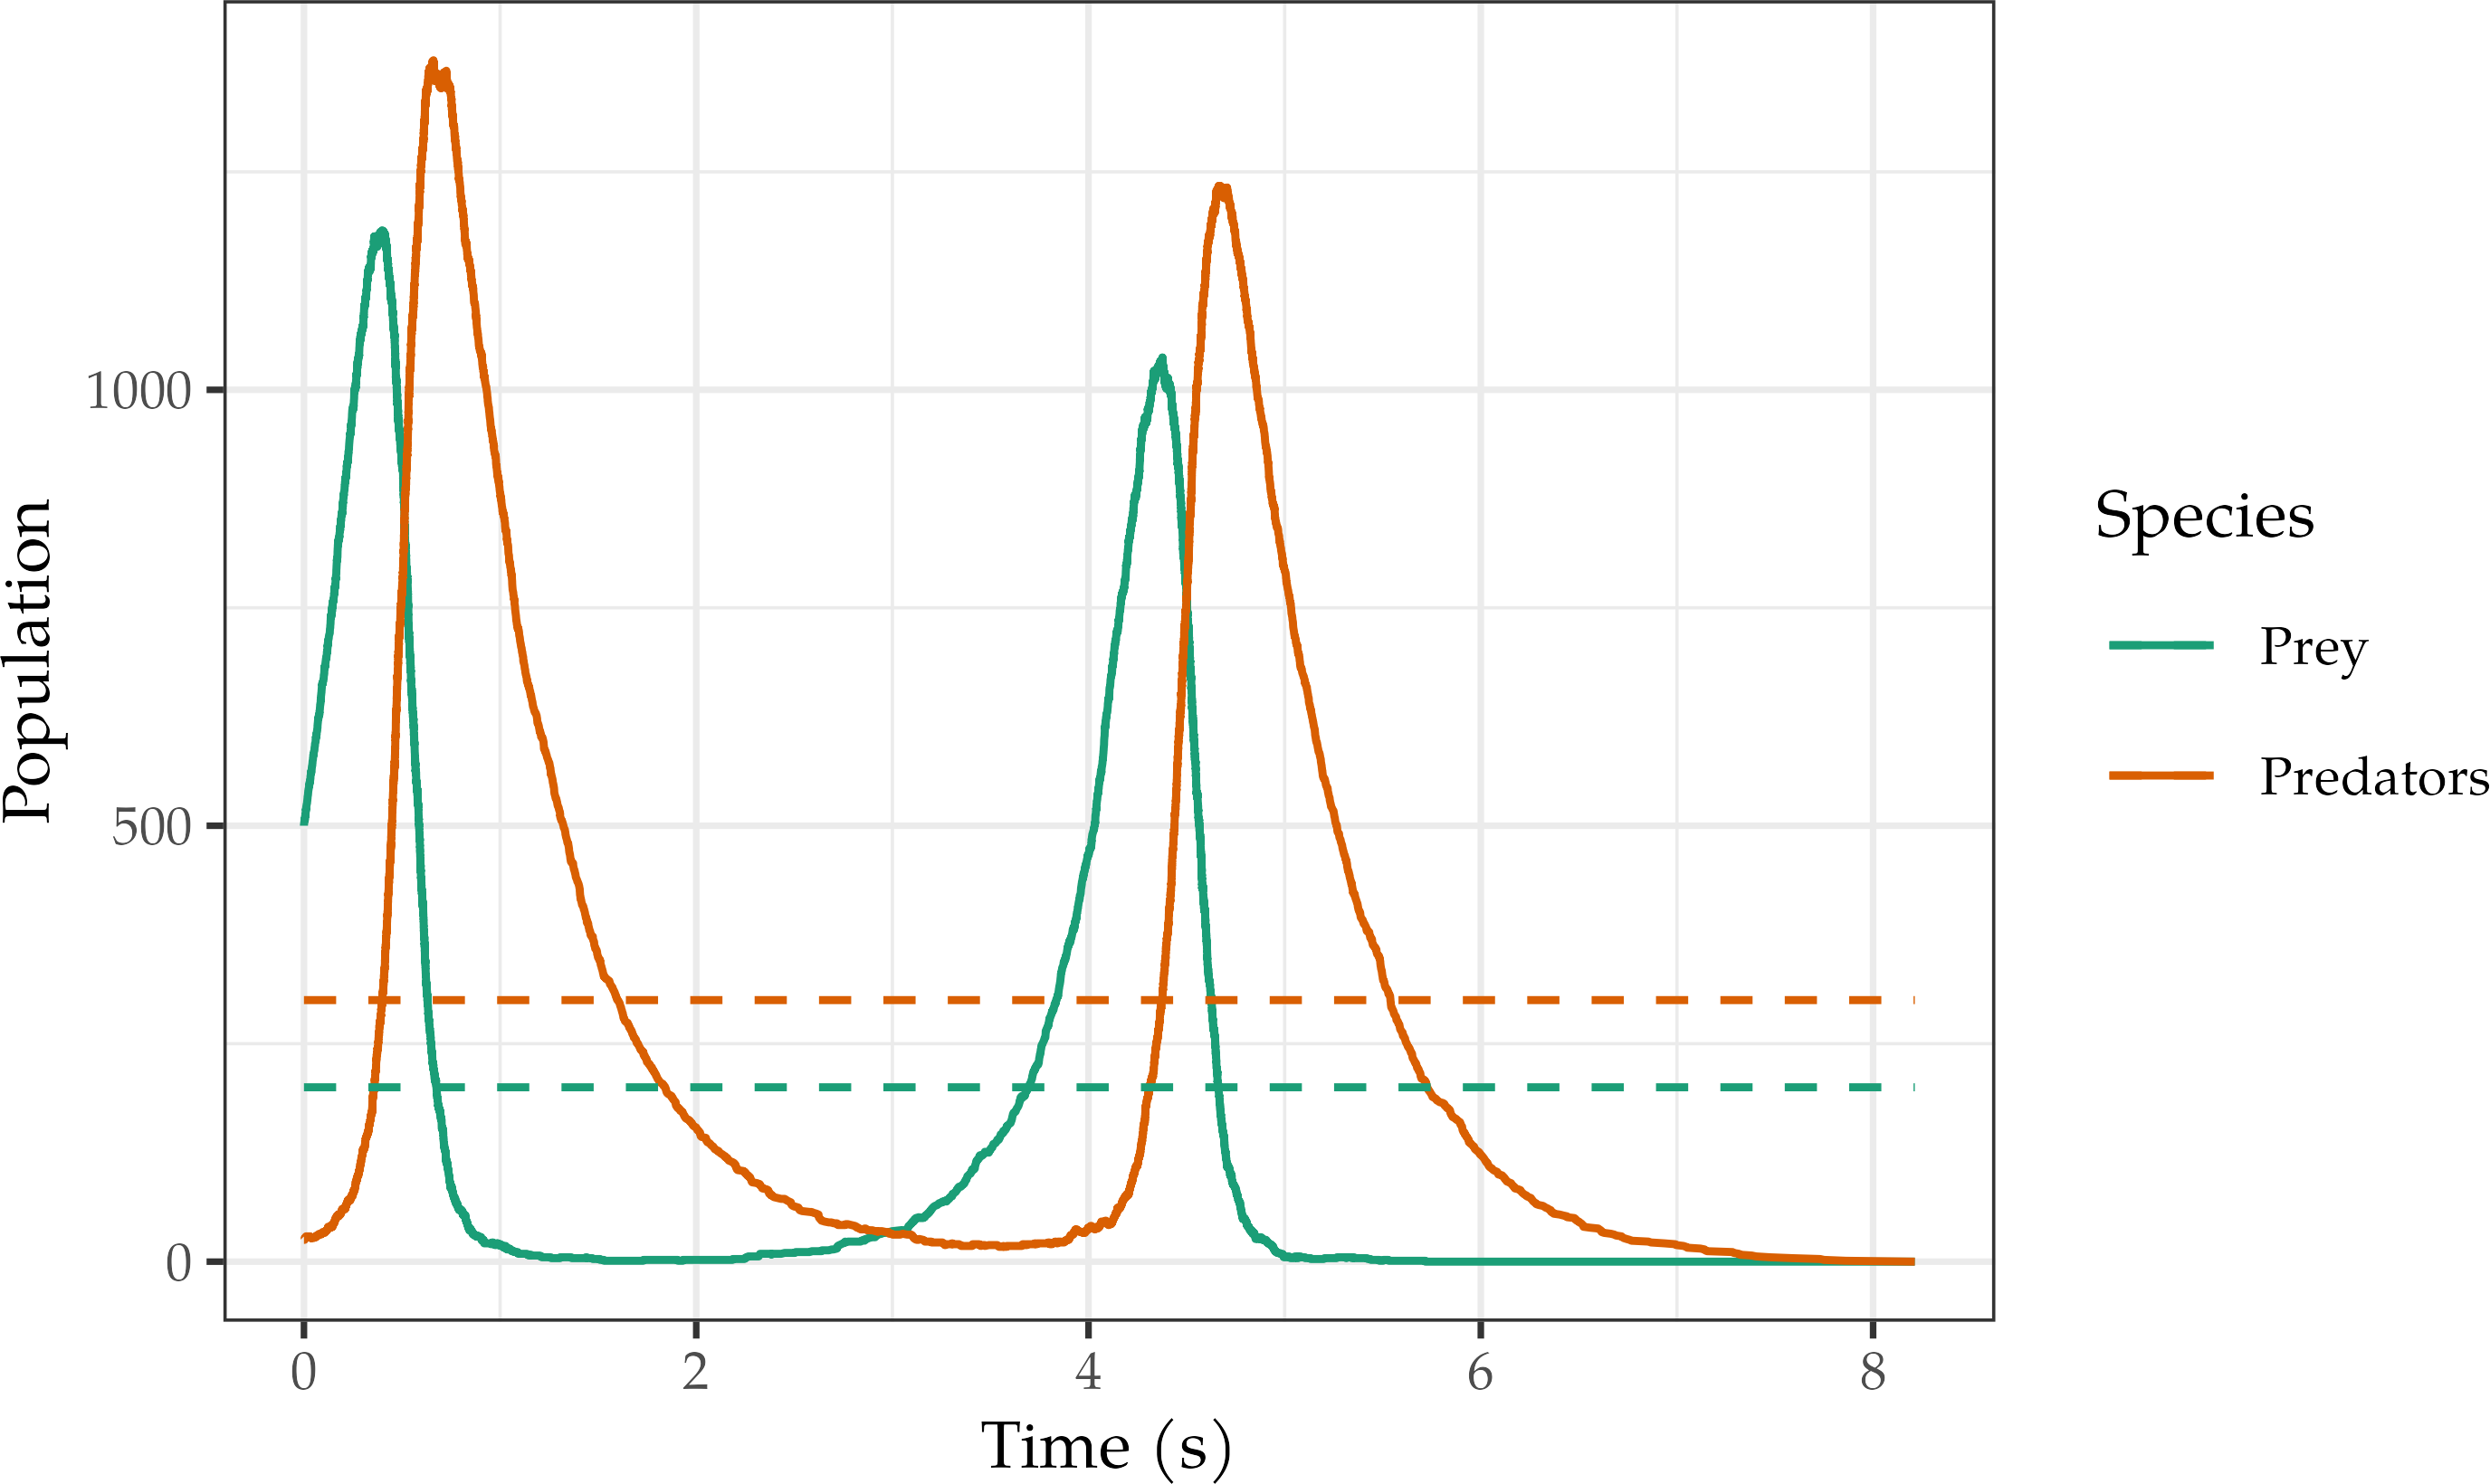
\includegraphics{img/071d.png}
  \caption{simulation of the Lotka--Volterra model with $k_{1} =
    \qty{3}{\per\second}$, $k_{2} = \qty{0.01}{\per\second}$ and $k_{3} =
    \qty{2}{\per\second}$.}
  \label{fig:071d}
\end{figure}

\section{Brusselator model}

\begin{figure}
  \centering
  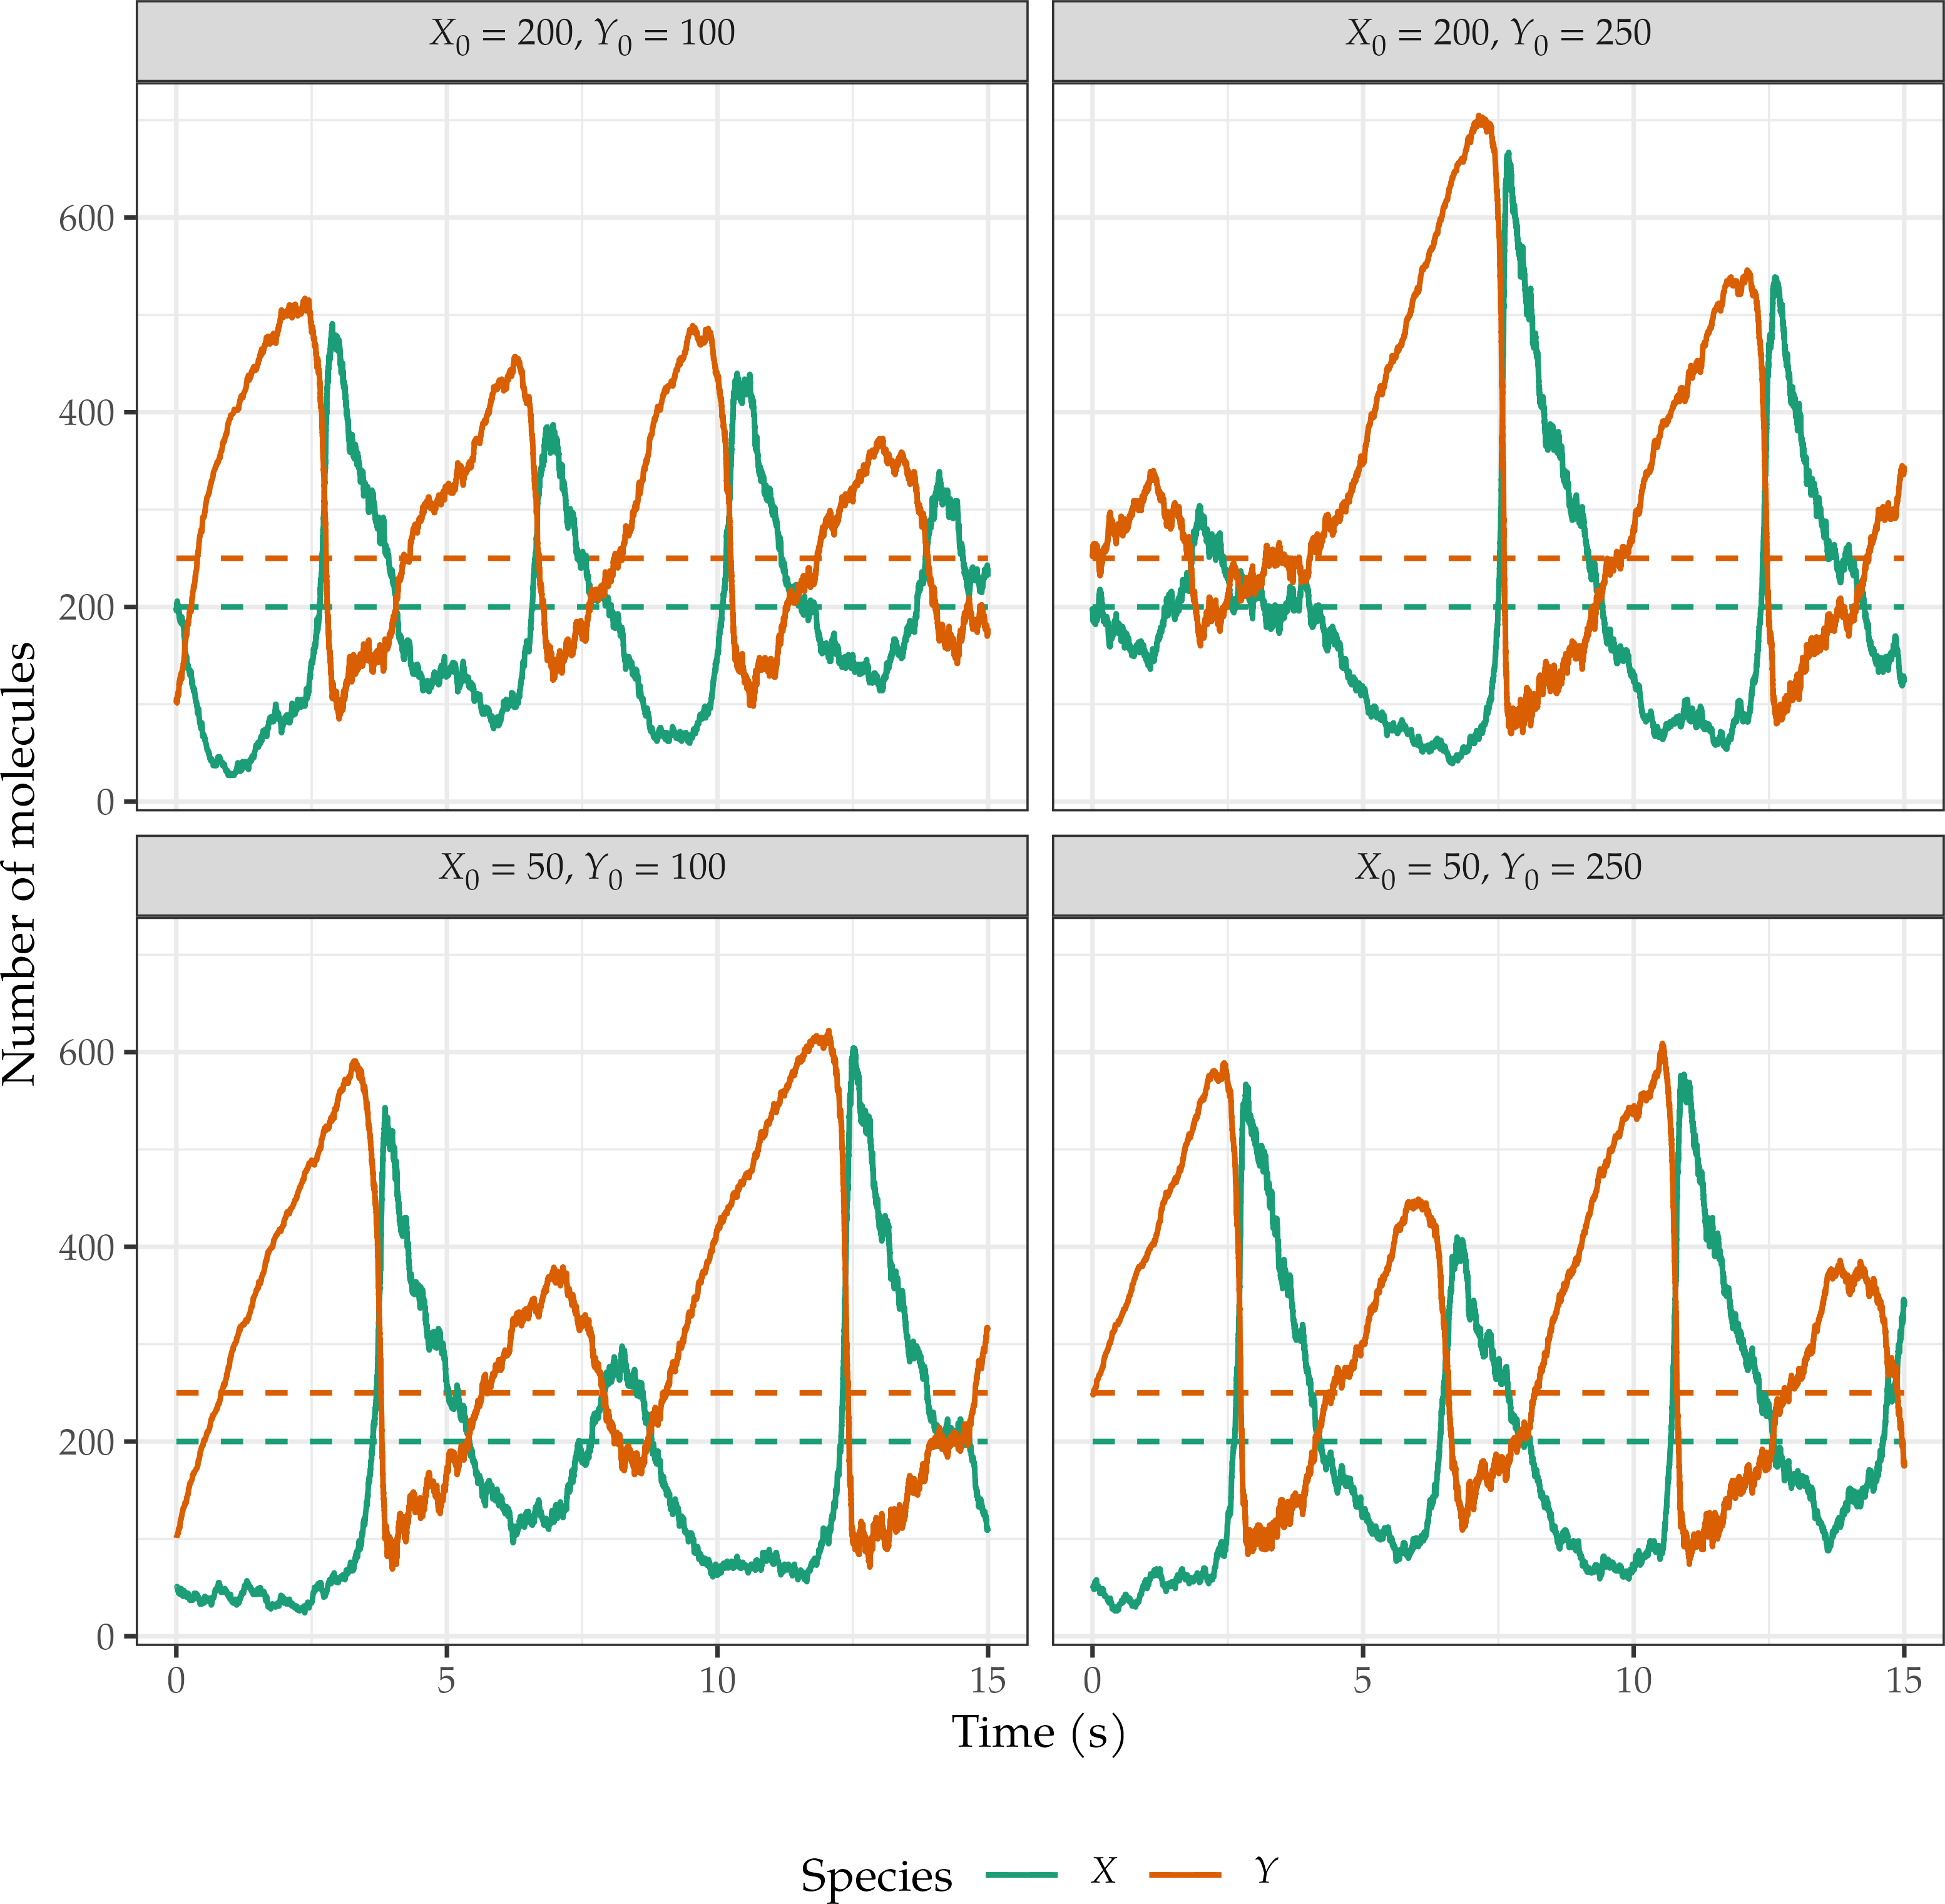
\includegraphics{img/072a.png}
  \caption{first set of Brusselator simulations, with $a =
    \qty{2}{\per\second}$, $b = \qty{5}{\per\second}$ and volume $\Omega =
    \num{e2}$. The initial conditions are reported above each plot and the
    stationary solution $(a \Omega, a \Omega / b)$ is highlighted with dashed
    lines.}
  \label{fig:072a}
\end{figure}

\begin{figure}
  \centering
  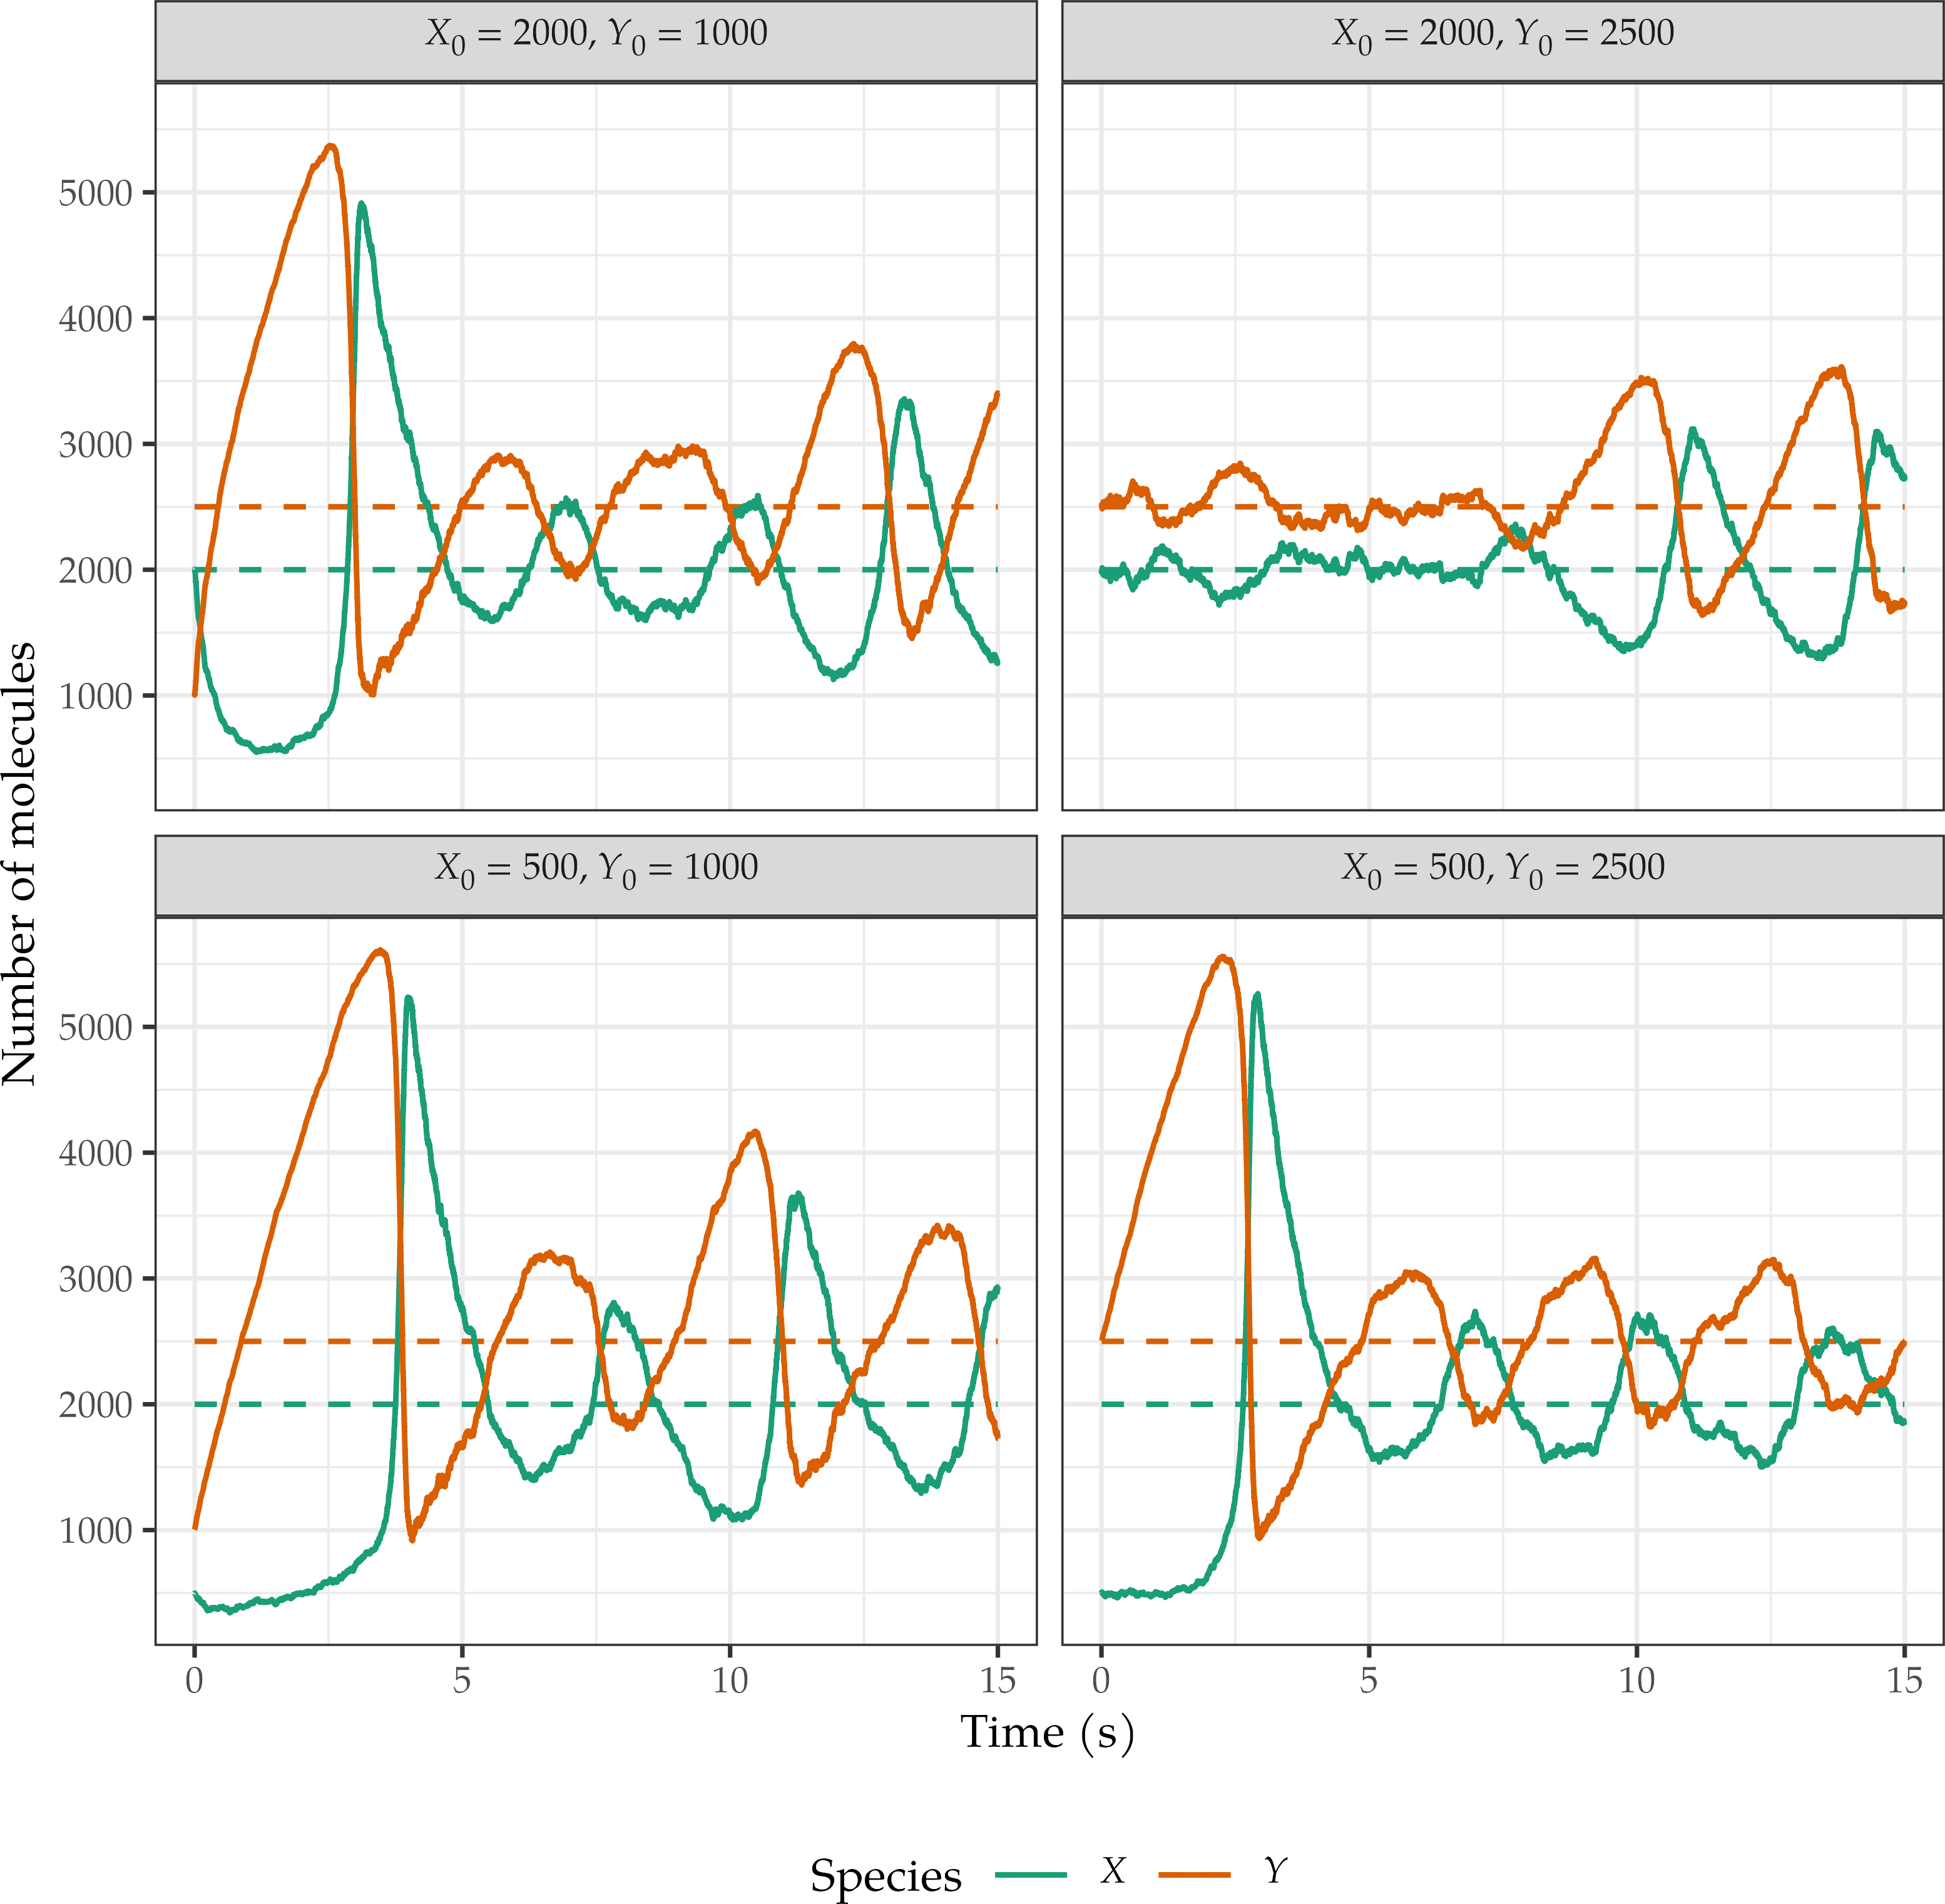
\includegraphics{img/072b.png}
  \caption{first set of Brusselator simulations, with $a =
    \qty{2}{\per\second}$, $b = \qty{5}{\per\second}$ and volume $\Omega =
    \num{e3}$. The initial conditions are reported above each plot and the
    stationary solution $(a \Omega, a \Omega / b)$ is highlighted with dashed
    lines.}
  \label{fig:072b}
\end{figure}

\begin{figure}
  \centering
  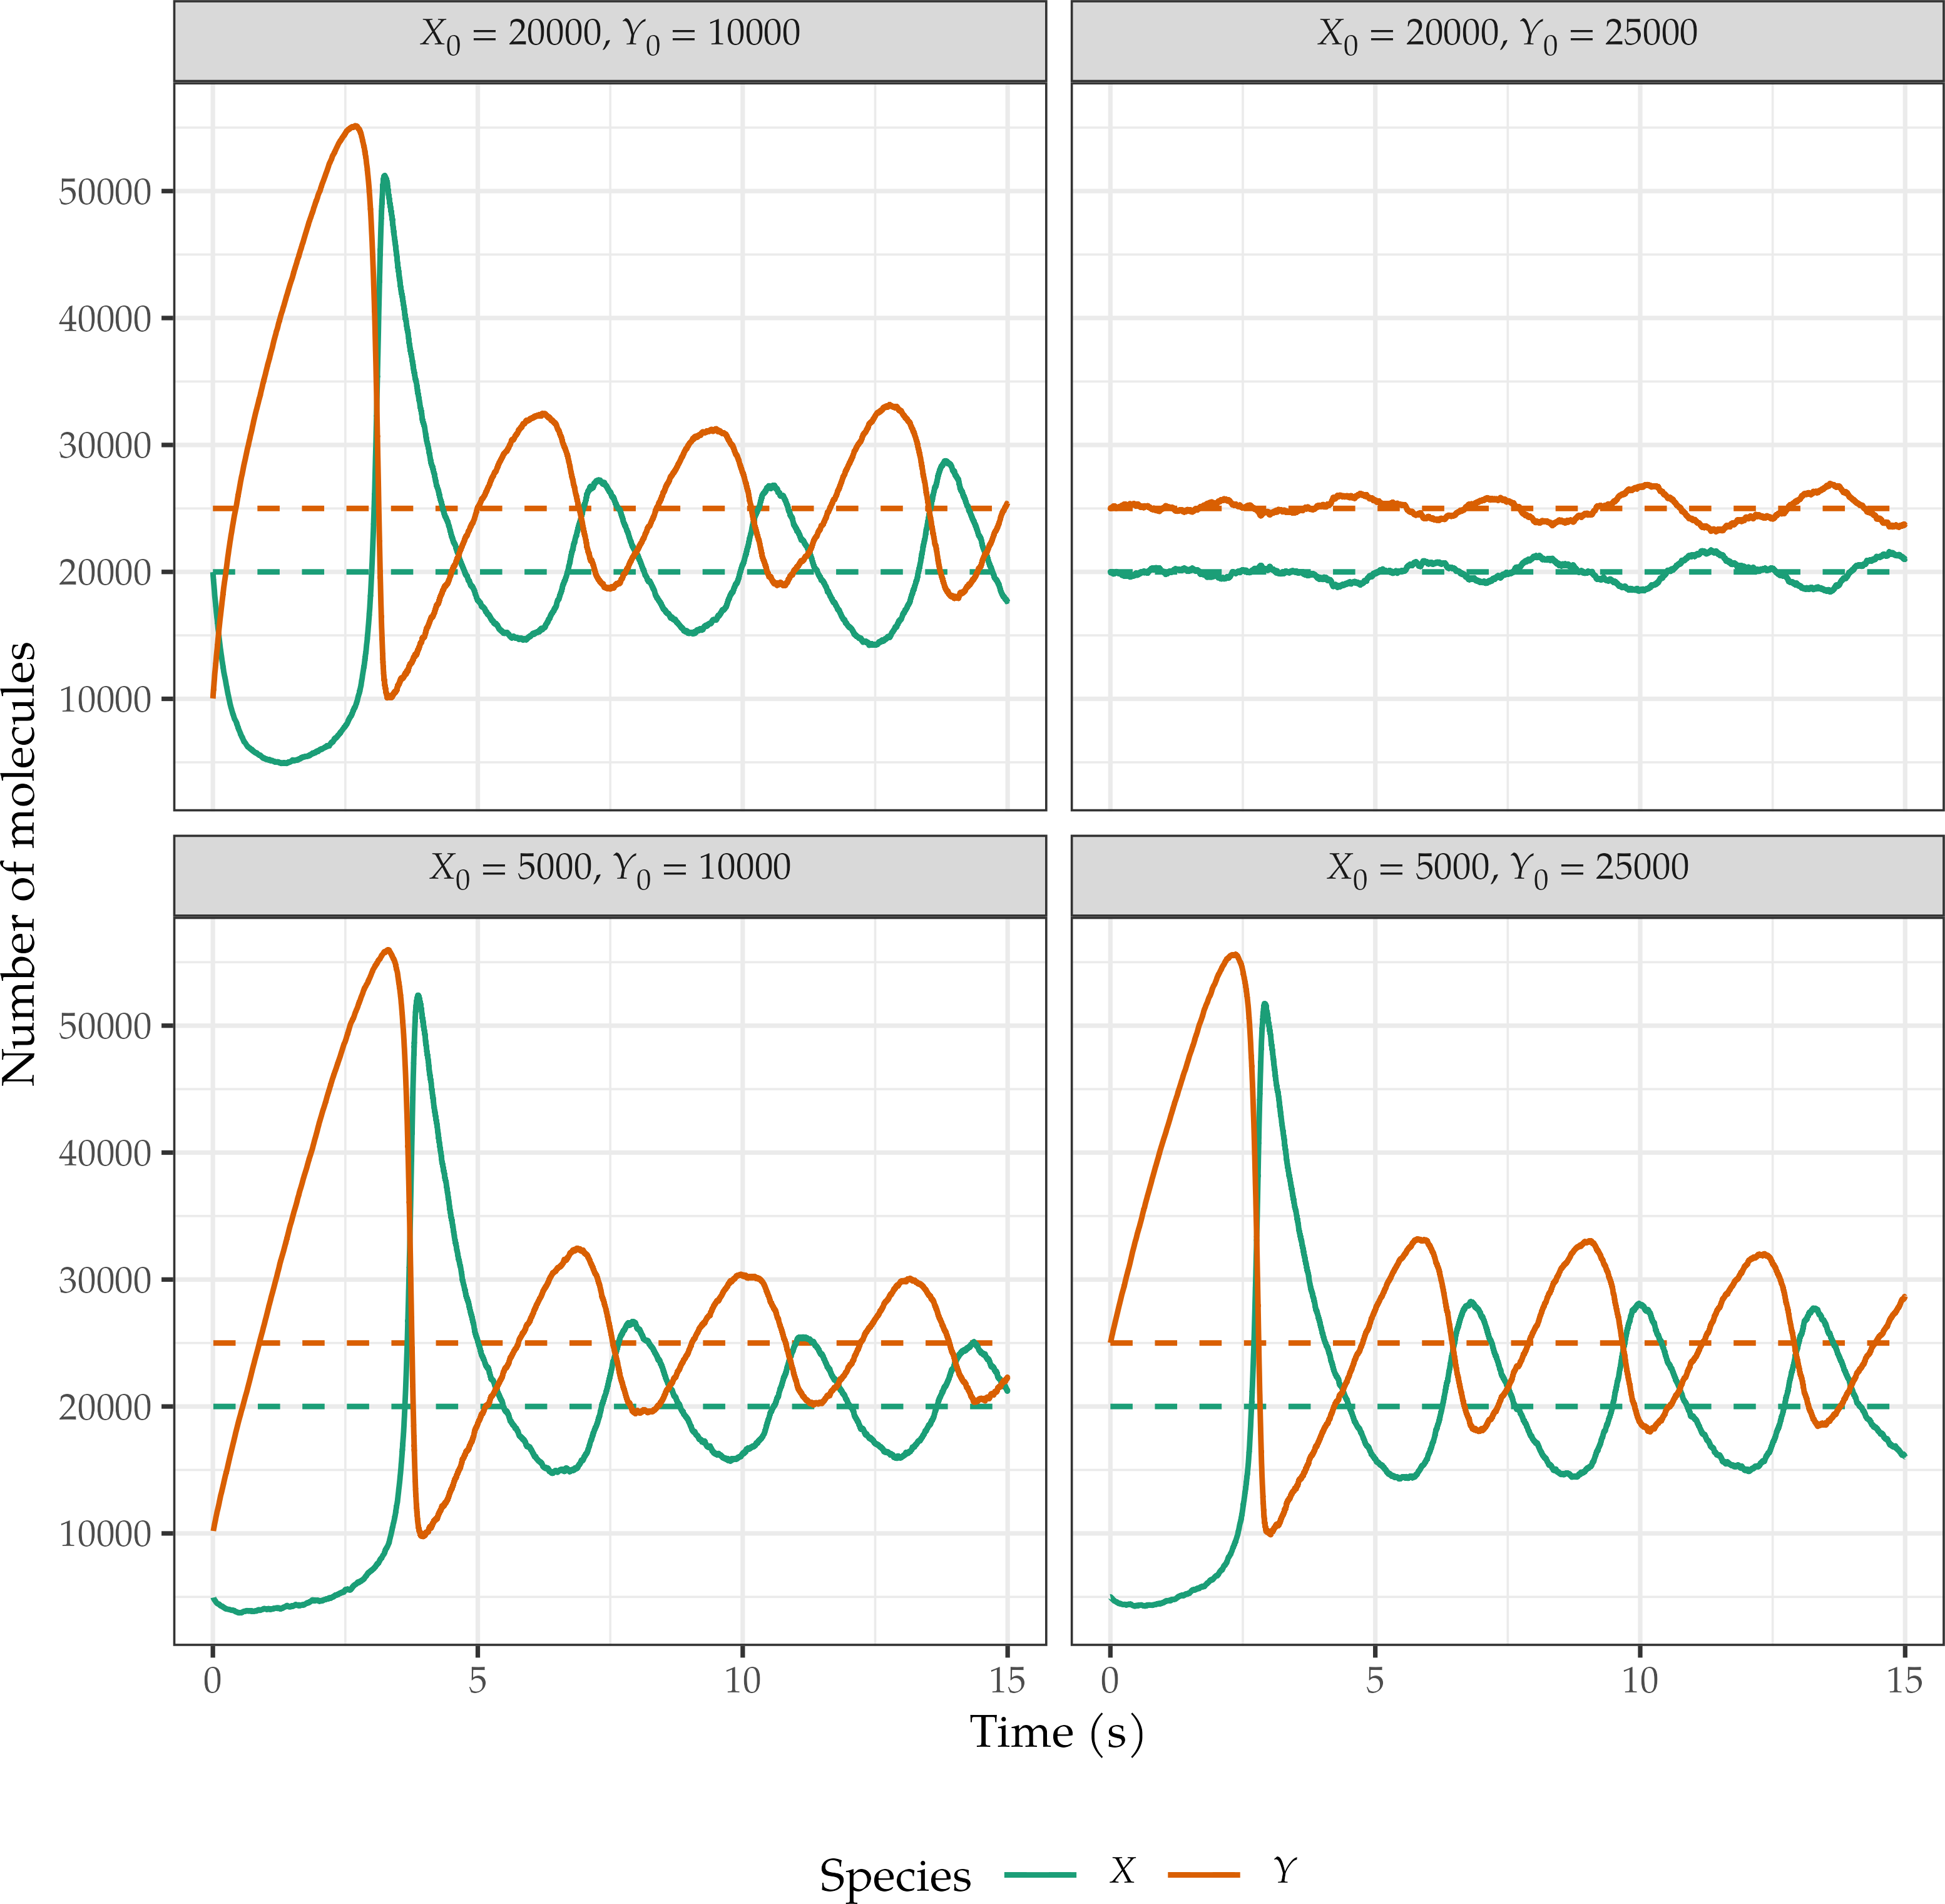
\includegraphics{img/072c.png}
  \caption{first set of Brusselator simulations, with $a =
    \qty{2}{\per\second}$, $b = \qty{5}{\per\second}$ and volume $\Omega =
    \num{e4}$. The initial conditions are reported above each plot and the
    stationary solution $(a \Omega, a \Omega / b)$ is highlighted with dashed
    lines.}
  \label{fig:072c}
\end{figure}
